\newpage
\subsection{Componentes da irradiação solar na produção de energia}

As nuvens são o principal fator modulador da radiação solar que incide na superfície em razão de suas propriedades óticas que produzem um espalhamento eficiente da radiação solar. O espalhamento da radiação solar por nuvens depende de sua espessura ótica, da distribuição de tamanhos das gotículas, do conteúdo e do estado físico da água \cite{PALTRIDGE}, características estas que variam de acordo com o tipo de nuvem \cite{atlas2017}.

A irradiância solar (W/m²) que incide em uma superfície é composta por suas componentes direta e difusa. A irradiância solar direta apresenta direção de incidência na linha imaginária entre a superfície e o Sol e representa a parcela que não sofreu os processos radiativos de absorção e espalhamento que ocorrem na atmosfera. A terminologia adotada por \cite{atlas2017} é a seguinte:

\begin{itemize}
  \item \textbf{Irradiância extraterrestre ($G_0$)} é a taxa de energia incidente por unidade de área em um plano horizontal imaginário situado no topo da atmosfera. É também conhecido como irradiância no topo da atmosfera ou GTOA.
  
  \item \textbf{Irradiância direta normal ($G_n$)} também conhecida como DNI, é a taxa de energia por unidade de área proveniente diretamente do Sol que incide perpendicularmente à superfície.
  
  \item \textbf{Irradiância difusa horizontal ($G_{dif}$)} é a taxa de energia incidente sobre uma superfície horizontal por unidade de área, decorrente do espalhamento do feixe solar direto pelos constituintes atmosféricos (moléculas, material particulado, nuvens, etc.)
  
  \item \textbf{Irradiância direta horizontal ($G_{dir}$)} é a taxa de energia por unidade de área do feixe solar direto numa superfície horizontal. Pode ser determinada como o produto entre a irradiância direta normal (DNI) e o cosseno do ângulo zenital solar. Irradiância global horizontal (G): é a taxa de energia total por unidade de área incidente numa superfície horizontal. A irradiância global é dada pela soma $G = G_{dif} + G_{dir} ou G = G_{dif} + G_n cos(\theta z)$ onde $\theta z$ é o ângulo zenital.

  \item \textbf{Irradiância no plano inclinado ($G_{i}$)} é a taxa de energia total por unidade de área incidente sobre um plano inclinado na latitude do local em relação à superfície da Terra.

\end{itemize}

A Figura \ref{fig:irradiacao_coceito} ilustra a irradiância assim que atinge a atmosfera e seu espalhamento e demostra as componentes da irradiação solar.

\begin{figure}[ht]
    \centering
    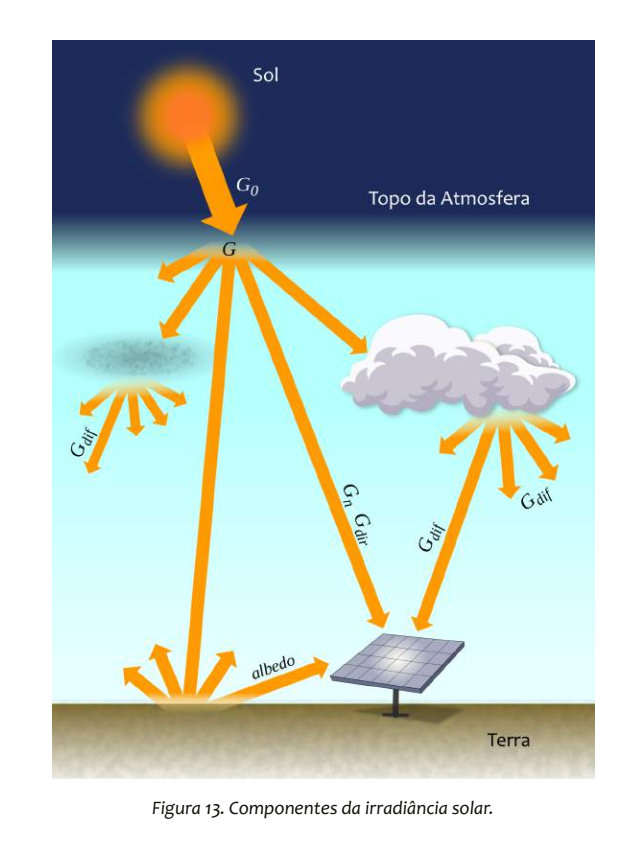
\includegraphics[width=0.45\textwidth]{./Figuras/irradiacao_coceito.png}
    \caption{Componentes da irradiância solar.}{Fonte: \cite{atlas2017}}
   \label{fig:irradiacao_coceito}
\end{figure}